\documentclass{article}
\usepackage[utf8]{inputenc}
\usepackage{amssymb}
\usepackage{tikz}
\usepackage{amsmath}
\usepackage{relsize}
\usepackage{mathtools}
\usepackage{textcomp}
\usepackage{eurosym}
\usepackage{amssymb}
\usepackage{systeme}
\usepackage{mathtools}

\title{Literature Review}
\author{Roman Oort}
\date{\today}

%%% PERSONAL SHORTCUTS
\DeclareMathOperator*{\plim}{plim}
\newcommand{\T}{\textbf{T}}
\newcommand{\Tij}{\textbf{T}_{ij}}
\newcommand{\Soc}{(\T(n))^{\infty}_{n=1}}
\newcommand{\beli}[3][2]{p_{#2}^{(#3)}}
\newcommand{\belvec}[2]{\textbf{p}^{(#2)}}

\begin{document}

\maketitle

\tableofcontents

\newpage

\section{Literature Review}
\subsection{Social Learning}
Social learning is a field of study used in various different disciplines, ranging from economy to psychology, concerning the process of changing beliefs in groups \cite{reed2010sociallearning}. Research in this field is dedicated to determining how individuals, and groups as a whole, change their beliefs and actions based on beliefs and actions of those around them. Many models have been proposed to formalize this process \cite{golub2017learning}, with the DeGroot model being one of the most prominent \cite{degroot1974concensus}.

\subsection{DeGroot Model}
\subsubsection{Agent Interaction}
A DeGroot model consists of a finite set of $N=\{1, 2, ..., n\}$ of agents all interacting with each other and passing information. The $n \times n$ \emph{interaction} matrix $\T$ describes the nature of these interactions: whose opinions are heeded by whom, and how much so. If the entry $\Tij > 0$ it indicates that agent $i$ listens to agent $j$, and the value of this entry determines how much weight agent $i$ places on agents $j$'s opinion: the higher this value the more important $j$'s opinion is to $i$. It is important to note that $\T$ is a positive matrix, meaning it is not possible for an agent to place a negative weight on another agents opinion, they are only ever capable of ignoring other agents, or agreeing with them in some manner. 

Furthermore, the weight matrix $\T$ is a row-stochastic matrix, meaning that its rows sum to one:
\begin{align*}
    \sum_{j=1}^{n} \Tij = 1
\end{align*}

Finally, the matrix $\T$ is not necessarily symmetrical, making it entirely possible for an agent $i$ to hold the opinion of agent $j$ in high regard, while in return $j$ thinks very little of $i$'s opinion, or not even anything  at all.

\newpage

\subsubsection{Belief \& Learning}
\label{beliefs}
As mentioned before, the DeGroot model is a model used to simulate social learning, and is often referred to as a form of \textit{naive social learning}. This means that this model simulates the development the beliefs of the agents present in the network, as time progresses, but the updating rule at each time-step is a very simple rule and is therefore called naive.

The belief of an agent $i \in N$ at a time $t \in \{0, 1, 2, ...\}$ is denoted as $p_{i}^{(t)}$, where this belief is taken as a real number on the interval $[0, 1]$. At the start of the process, $t=0$, each agent $i$ is given a personal belief, through a private signal:
\begin{align*}
    \beli{i}{0} = \mu + e_i
\end{align*}
where $\mu$ is a real number, again on the interval $[0, 1]$, assumed to be the true state of the network, and $e_i$ is the random, zero mean, noise of agent $i$'s signal. \newline
The beliefs of all agents in the network, are aggregated into the belief vector $\textbf{p}^{(t)}$, where the $i$th entry corresponds to the belief of agent $i$, at time $t$.

As time progresses the agents in the network update their own belief based on the beliefs of the agents around them, using the following updating rule:
\begin{equation}
    \label{updating:standard}
    \textbf{p}^{(t)} = \T\textbf{p}^{(t-1)}
\end{equation}
which means that an agent $i$'s opinion, at time $t$, is simply the matrix multiplication of the interaction matrix and the belief vector at time $t-1$. This makes the update rule for an agent $i$ in the network the following:
\begin{align*}
    \beli{i}{t} = \sum_{j=1}^{n}\Tij\beli{j}{t-1}
\end{align*}
which simply amounts to the weighted sum of the beliefs of all neighbours of agent $i$ in the network, where agent $i$'s neighbours are those agents $j$ in the network to whom $i$ listens.

Furthermore, it is possible to compute the belief vector $\textbf{p}^{(t)}$, without computing the belief vector at every preceding $t^\prime < t$, the formula for which can be derived from equation \ref{updating:standard}, as follows:
\begin{align*}
    \textbf{p}^{(t)} &= \T\textbf{p}^{(t-1)} \\
    &= \T\T\textbf{p}^{(t-2)}\\
    &= \T^2\textbf{p}^{(t-2)}\\
    &= \T^3\textbf{p}^{(t-3)} \\
    &= \T^{t}\textbf{p}^{(0)}
\end{align*}

\newpage

\subsubsection{Convergence}
\label{convergence}
As we are interested in the spread of information through the network, and whether the agents in a network will learn the supposed true state of the world, an important notion is the concept of \emph{convergence}. A matrix \textbvf{T} is said to be convergent if:
\begin{equation*}
    \lim_{t\to\infty} \T^t\textbf{p}
\end{equation*}
exists for all $\textbf{p} \in [0, 1]^n$. That is to say, as time progresses sufficiently, the beliefs of the agents, independent of their starting signal, approach a constant value and no longer change.

Another important property is \emph{aperiodicity}, which concerns cycles: paths through the network that start and end at the same agent. A network is said to be aperiodic if the largest common divisor of the length of all cycles in the network is no more than 1. This condition is automatically satisfied as long as there is at least one agent present in the network who has a link to themselves, as this creates a cycle of length one, which only has one as a divisor, ensuring there can be no larger common divisor.

A final notion important in the convergence of social networks is \emph{connectedness}. When applied to undirected networks, in which a link between two agents works both ways, a network is said to be connected when there exists some path between any two agents $i$ and $j$. However, when applied to \emph{directed} networks this notion changes slightly, and can be divided in two distinct notions, more specifically, a connected directed network can be either \emph{weakly} or \emph{strongly} connected. A directed network is said to weakly connected if there exists some undirected path between any two agents in the network. However, if there also exists a \emph{directed} path between any two agents, a directed network is said to be strongly connected.

Now, assuming that \T, is the interaction matrix of a strongly connected network, the following three statements are equivalent:
\begin{itemize}
    \item[-] $\T$ is convergent
    \item[-] $\T$ is aperiodic
    \item[-] There is some unique left eigenvector, \textbf{s}, of \T, corresponding to the eigenvalue $\lambda=1$, such that, for every \textbf{p}$\in [0,1]^n$, and every agent $i$,
    \begin{align*}
        (\lim_{t\to\infty}\T^t\textbf{p})_i = \textbf{sp}
    \end{align*}
\end{itemize}

 This last eigenvector property does not only give a definition of convergence, but it also provides the actual convergent belief of the network, which is nothing more than a multiplication of the influence vector \textbf{s} and the belief vector \textbf{p}. Finally, this also shows that when a network converges the convergent belief will be the same for all agents, that is to say that as time progresses eventually all agents will hold the same opinion.

\newpage

\subsubsection{Wisdom of Crowds}

Having established the convergence property for social networks it becomes possible to look towards the notion of wisdom, central in \cite{golub2010naive}. They defined wisdom to mean that a given network not only converges, but converges to the assumed true state of the model, $\mu$, looking in particular in the context of large societies. This means they are looking at networks where the number of agents in the network $n\to\infty$.

To encapsulate the idea of large societies, providing insight in the behaviour of these models as the participating number of agents becomes sufficiently large, limiting statements with regard to the number of agents are used. A society is defined as a sequence of networks, indexed by the number of agents in the network, $n$: $\Soc$. This means that the entry $\textbf{T}(n)$ is the interaction matrix of the network in the sequence with $n$ agents, where $\textbf{T}(n)_{ij}$ is used to denote the entry $(i,j)$ in this specific sequence. A similar method of indexing is applied to all previously discussed properties of these networks, i.e.: belief vectors, influence vectors.

The beliefs of the agents are generated using the same mechanism described in section \ref{beliefs}, i.e.: independently distributed zero mean error terms added to the assumed truth, where $\beli{i}{t}(n)$ is used to indicate the belief of agent $i$ at time $t$ in a network with $n$ agents. Under the assumption that every network in our given sequence converges, we write the convergent belief of an agent $i$, that is to say the belief as $t \to\infty$, as $\beli{i}{\infty}(n)$, as described in \ref{convergence}.

Using these notations a sequence $\Soc$ is deemed to be wise if:
\begin{equation}
    \label{wisdom:equation}
    \plim_{n\to\infty}\max_{i \leq n}|\beli{i}{\infty}(n) - \mu| = 0
\end{equation}
That is to say, a sequence of network is wise if, as $n$ becomes sufficiently large, the convergent belief of \emph{every} agent in the network is equal to the truth, which, using the fact that the convergent belief can be computed using the influence vector \textbf{s} can be rewritten as:
\begin{equation}
    \label{wisdom:influence}
    \plim_{n\to\infty} \textbf{s}(n)\textbf{p}^{(0)}(n) = \mu
\end{equation}
which holds if and only if $s_{1}(n) \to 0$, where $s_1(n)$ is the first entry in the \emph{ordered} influence vector \textbf{s}. In other words, a sequence of networks if wise if and only if the influence of the most influential agent tends to zero, as $n$ becomes sufficiently large.

\newpage

\subsection{Obstructions to Wisdom}

\subsubsection{Prominent Families}

One general obstacle to the convergence to wisdom is similar to requirement of vanishing influence of individual agents. Namely, the existence of groups in the network that are disproportionally influential over other groups.
A general obstacle to the convergence to wisdom is presence of groups that are disproportionally influential when compared to other groups in the network.

To reason about groups and the influence between them a definition of the influence of a groups is necessary, as all previously mentioned notions of influences were applied only on the scale of individual agents. Let $B$ and $C$ be two groups in the network s.t. $B \subset N$ and $C \subset N$ and $B \cap C = \emptyset$, where $N$ is the set of all agents in the network, then the weight that group $B$ places on $C$ is defined as follows:
\begin{equation}
    \textbf{T}_{B, C} = \sum_{i\in B}\sum_{j \in C} \Tij
\end{equation}
Simply put: the weight of a group $C$ on another group $B$ is simply the sum of all incoming links from agents in $B$ to agents in $C$.

Another measure used to describe the influence of groups is the prominence of a group, which is a measure of the influence of a group $B$ over the entire network \textbf{T}, rather than another group in the network.
 A network is said to be prominent, at a given $t$, if every agent $i \notin B$ in the network listens to some agent $j\in B$, at that $t$.
A group $B$ is therefore said to be prominent in $t$ steps relative to a network \textbf{T} if, for every $i \notin B$, $(\textbf{T}^{t})_{i,B} > 0$. An important property based on this notion is the $t$-step prominence of B relative to \textbf{T}: 
\begin{equation}
    \pi_B(\textbf{T}; t) = \min_{i\notin B} (\textbf{T}^{t})_{i,B}
\end{equation}
This is the smallest weight that is placed on some agent in the group $B$, by some agent $i\notin B$. Therefore this value will only be larger than zero for any values $t \geq t^{\prime}$, where $t^{\prime}$ is the smallest t for which
the group $B_n$ is prominent relative to the network.
\newline

However, these definitions of groups are defined only on single networks while, in the context of wisdom, we are interested in sequences of networks. The notion of groups can be slightly expanded to be useful in the context of societies. For this end we define a family as a sequence of groups $(B_n)$, where each $B_n \subset \{1, ..., n\}$, such that each group in the sequence is a subset of the agents present in the network of size $n$.

Having extended the notion of groups to the context of societies the measure of prominence can be expanded in a similar manner. Namely, a family $(B_n)$ is said to to uniformly prominent relative to $\Soc$ if there exists a constant, $\alpha$, and there is a $t$ such that $B_n$ is prominent in $t$ steps relative to $\T(n)$, and $\pi_B(\textbf{T}; t) \geq \alpha$, for every $n$. In other words, for a family $B_n$ to be uniformly prominent it has to have a minimum influence greater than $\alpha$ over each individual agent $i$ outside of $B_n$, at every size $n$ of the society.

\noindent Finally, a family $(B_n)$ is called finite if there exists some $q$ such that:
\begin{equation*}
    \sup_n |B_n| \leq q
\end{equation*}
Or, in other words, a finite family is a family that has a finite upper bound on its members.

Now, it is the case that the disproportional influence of groups can cause a network no longer to be wise, namely, the presence of finite, uniformly prominent family relative to the society $\Soc$, prevents this society from becoming wise.

\subsubsection{Non-cooperative Agents}
\label{non-coop}
Another factor capable of preventing wisdom in a network is the presence of a non-cooperative agent in the network \cite{amir2021robust}. That is to say, an agent in the network who does not adhere to the regular updating mechanics, deliberately spreading misinformation to its neighbours. The presence of even one of these non-cooperative agents in  the network is enough to prevent wisdom in the network, assuming the private belief of this agent is not equal to the assumed truth. Even though a network may satisfy all the necessary conditions required for wisdom this one agent not playing by the rules will steer the network away from the convergent belief. In fact, not only will this agent prevent the other agents from converging to the truth, it also ensures all other agents converge to its own belief.


When a non-cooperative agent, or bot \cite{amir2021robust}, is present in the network instead of converging towards wisdom, in a network of sufficient size, the opinions of the agents will converge towards the opinion of the non-cooperative agent in the network. 

\subsubsection{Structural Obstructions}

Finally there are some obstructions that prevent the occurrence of wisdom in a given society that are more dependent on the actual structure of the network rather than the weights on the links or adherence to the updating rules. One example of such a structure is a specific network, called a star network. A star network is a fully connected network in which there is one agent which has a connection to every other agent in the network, while every other agent only has a connection to this one agent. These networks are called star networks because, when visualized, obtain a star-like shape, an example of which can be seen in figure \ref{network:star} below.

\begin{center}
    \begin{figure}[!htbp]
        \centering
        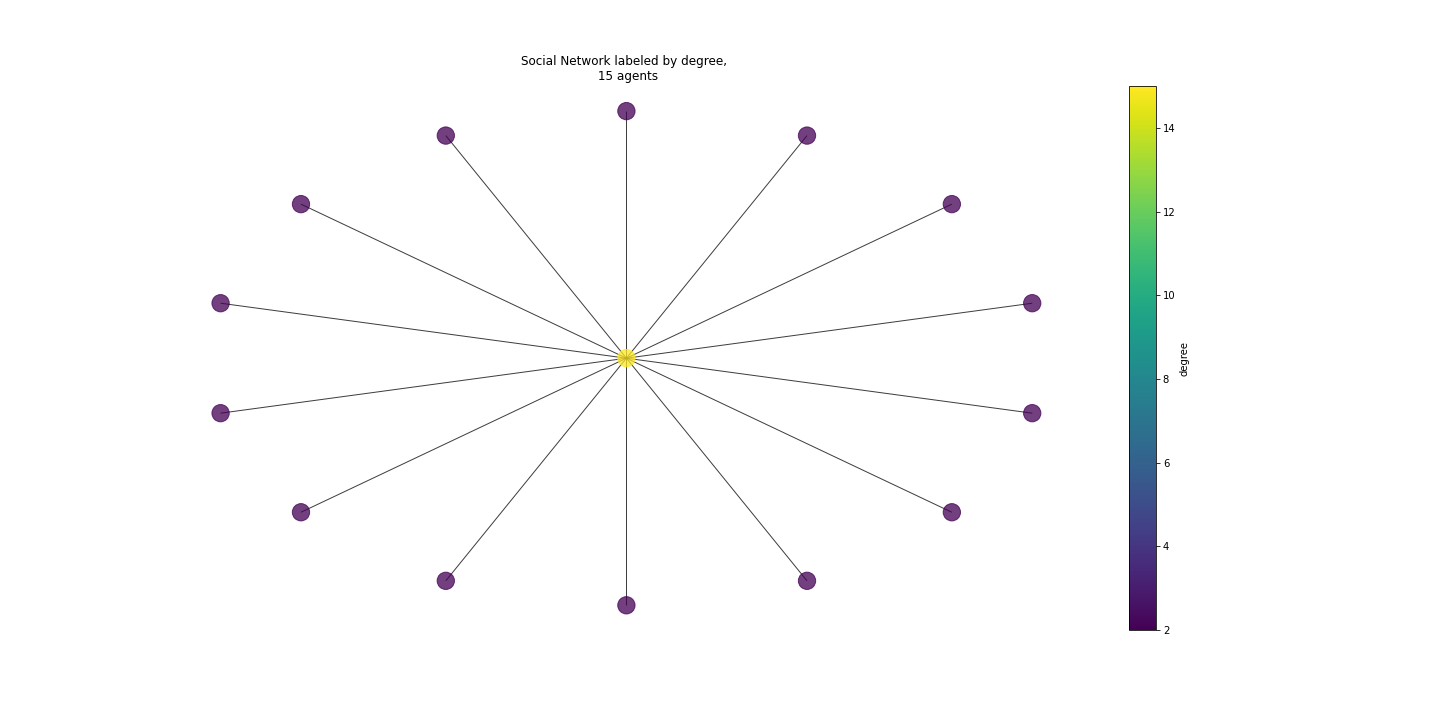
\includegraphics[width=\textwidth]{ThesisKI/Images/DegreeStarGraph.png}
        \caption{Degree Distribution, Instant}
        \label{network:star}
    \end{figure}
\end{center}
\newpage
Here the network is shown for $n=15$, but this specific shape of network can be extended to any size $n$, using the same principle of one agents who is connected to every other agent, with the other agents only connecting with this center agent. As a consequence this one agent in the center has a disproportional amount influence when compared to the other agents. Therefore, if this agent's initial belief diverges enough from the truth the condition for wisdom described in \ref{wisdom:influence} is no longer satisfied.

However, networks where there is not a single agent with a disproportionate amount of connections can still disrupt the wisdom of a network. An example of this is the unbalanced line network described by \cite{golub2010naive}, where the network forms a line, where each agent $n$ places a weight of $\delta \in (0, \frac{1}{2})$ on the agent $n+1$, and places a weight of $1-\delta$ on the agent $n-1$. The two agents at the start and end of this line, $1$ and $n$, place a weight on their own opinion of $1-\delta$ and $\delta$ respectively. In this case the influence of agent $1$ can become arbitrarily close to $1$ by choosing $\delta$ to be sufficiently small, once again violating \ref{wisdom:influence}, preventing wisdom.

So, as there are structural obstructions to the wisdom of a society, so too are there some structural conditions that need be satisfied to ensure wisdom. Determining these conditions requires some more notions about the structures of the network, like the concept of balance. For a network to be considered balanced there must be a sequence $j(n) \to \infty$, such that if $|B_n| \leq j(n)$ then:
\begin{equation}
    \sup_n \frac{\T_{B^c_n, B_n}(n)}{\T_{B_n, B^c_n}(n)} < \infty
\end{equation}

This notion captures the idea that a group cannot be too self-centered, that is to say, that it is influenced a disproportionately by agents outside said groups, while the group itself exerts very little influence on those agents. However this only needs to hold for groups smaller than indicated by the sequence $j(n) \to\infty$.
This property is a natural extension of the idea that one single agent should not be getting infinitely more weight than they are placing on other agents, but applied to groups rather than individual agents. \newline

However, balance alone is note enough to ensure a wise network. Another important, structural, measure is the minimal out-dispersion. This condition states that there exists some $q\in \mathbb{N}$ and $r > 0$, such that if $B_n$ is a finite group, $|B_n|\geq q$ and $\frac{|C_n|}{n}\to 1$, then $\textbf{T}_{B_n, C_n} > r$, as $n$ becomes sufficiently large. Simply put, this condition requires that any finite group of a give size must place a minimal amount of weight on a group consisting of nearly the entire network. This prevents specific groups from only focussing their attention inward and ignoring the vast majority of the network.

With these two condition in place it is possible to formulate a sufficient condition for wisdom, namely, that if $\Soc$ satisfies \emph{both} balance and minimal out-dispersion, it is wise.

\subsection{Variations}
As mentioned in \ref{non-coop} the presence of non-cooperative agents in the network is greatly disruptive for the ability of a network to attain wisdom. So much so, even, that only one non-cooperative agent is sufficient to prevent any network, regardless of size, from attaining wisdom. Furthermore, not only does this agent prevent wisdom, it also ensures that the final convergent belief of the network will be equal to its own belief, with regard for neither the initial beliefs of the agents, nor the assumed truth of the network. As the presence of even one such agent disrupts the wisdom of the entire network research is done on how to make the standard, \emph{naive}, DeGroot model more resilient to the presence of such non-cooperative agents.

\subsubsection{$\varepsilon$-DeGroot}

One such variation, specifically designed by \cite{amir2021robust} to combat the presence of such non-cooperative agents in the network, is called $\varepsilon$-DeGroot. This variation makes a small adjustment to the standard updating rule of the DeGroot model, in an attempt to achieve wisdom despite non-cooperative agents present in the network.

In the standard DeGroot model an agent's belief at time $t$ is simply the weighted sum of their neighbours' opinions, according to \ref{updating:standard}. In contrast, in the $\varepsilon$-DeGroot model, the parameter $\varepsilon$ is used as a threshold in the updating step to prevent agents from changing their belief drastically in a single time-step.
Instead of simply updating their current opinion, $x$, to the weighted sum of their neighbours' opinions, $y$, they check whether the difference between the two falls under the threshold before updating their opinion, changing the updating rule from \ref{updating:standard} to:

\begin{equation}
    \label{edegroot:updating}
  \beli{i}{t} =\Bigg\{
  \begin{matrix*}[l]
  y \text{ if } |\beli{i}{t-1} - y| \leq \varepsilon\\
  y^{\prime}\in\{y-\varepsilon, y+\varepsilon\}\text{ s.t. }|\beli{i}{t-1} - y^{\prime}|\text{ is minimized, otherwise}
  \end{matrix*}
\end{equation}
where $y = (\textbf{T}\textbf{p}^{t-1})_i$. This means that at each $t$ each agent $i$ does not indiscriminately change their opinion to the combined opinion of its neighbours', as under regular DeGroot mechanics. Rather, it checks whether the difference between this combined belief and its own, previous, belief, falls under a certain threshold, given by $\varepsilon$. If so, it takes this combined opinion, otherwise it changes its opinion to the closest of $\{y-\varepsilon, y+\varepsilon\}$. So, the larger $\varepsilon$ is chosen, the more an agent can change its opinion in a single updating step, and the smaller this $\varepsilon$ is chosen, the more this rule approaches the standard DeGroot updating process. After all, if $\varepsilon = 0$ the updating rule becomes:
\begin{equation*}
  \beli{i}{t} =\Bigg\{
  \begin{matrix*}[l]
  y \text{ if } |\beli{i}{t-1} - y| \leq 0\\
  y^{\prime}\in\{y\}\text{ s.t. }|\beli{i}{t-1} - y^{\prime}|\text{ is minimized, otherwise}
  \end{matrix*}
\end{equation*}

Using an updated metric for the learning process, called $(\delta, \rho)$-learning, which is achieved by that agent if their opinions falls with in $\delta$ of the assumed truth, $\mu$, with probability $1 - \rho$. On an infinite graph this condition is satisfied when all but a finite group of agents satisfy this condition. \newline

One thing to note is that the $\varepsilon$-DeGroot mechanics do not necessarily impose a hard limit on the change of opinion of an agent. After all, when the threshold is exceeded the updated is still based on the newly computed opinion, which could lay arbitrarily far away, on the interval $[0, 1]$, from the currently held opinion. Therefore an alternate approach to the $\varepsilon$-DeGroot dynamics would be to base the new opinion, should the difference between the currently held opinion and the newly computed one exceed the threshold, on the currently held opinion, rather than the 
newly computed one. In case the threshold is exceeded this would impose a hard limit on how much agents' opinion can change at once. This would change the updating rule as described in \ref{edegroot:updating} to:
\begin{equation*}
    \label{edegroot:alt}
    \beli{i}{t} =\Bigg\{
    \begin{matrix*}[l]
        y \text{ if } |\beli{i}{t-1} - y| \leq \varepsilon\\
        x^{\prime}\in\{\beli{i}{t-1}-\varepsilon, \beli{i}{t-1}+\varepsilon\}\text{ s.t. }|y - x^{\prime}|\text{ is minimized, otherwise}
    \end{matrix*}
\end{equation*}
In other words, should the difference between the new opinion and the previous opinion exceed the threshold, $\varepsilon$ is simply added to, or subtracted from, the current opinion, whichever is closest to the belief as computed through the standard updating rule.

\newpage

\subsubsection{Private Belief}

Another variation introduced by [FRIEDKIN AND JOHNSEN, 1999 GEREFD IN GOLUB 2017], permits each agent to hold on to persistent private belief. When updating each agent then not only considers the weighted sum of the beliefs of their neighbouring agents, but also take into account this private belief. Furthermore, this private belief does not change over time, but remains constant, making it distinct from an agents' link to itself, should this be present. This variation on the model changes the updating rule to the following:

\begin{equation}
    \beli{i}{t} &= (1-\alpha_i)(\textbf{T}\textbf{p}^{(t-1)})_i + \alpha_i b_i
\end{equation}
where $b_i$ is the private belief of an agent $i$, of course on the interval $[0, 1]$, and $alpha_i$ is the weight that said agent places on their private belief, also on the interval $[0, 1]$. In essence the updating rule becomes a weighted sum of the new belief, as computed through the standard updating rule, and an agent's private belief.

\subsubsection{Stochastic DeGroot}

One final variation on the standard DeGroot model that will be discussed is the \emph{stochastic} DeGroot model. Rather than keeping the interaction matrix $\textbf{T}$ constant as $t \to \infty$, the stochastic DeGroot model allows this matrix $\textbf{T}$ to change over time. This alleviates one of the main pitfalls of the standard DeGroot model, which supposes that each agent will never change the weight they place on the opinions of their neighbours. Instead a stochastic DeGroot model allows the weights to evolve over time. This changes the updating rule to the following:
\begin{equation*}
    \beli{i}{t} &=(\textbf{T}(t)\textbf{p}^{(t-1)})_i
\end{equation*}
The idea of the updating rules remains the same, the only difference being that the weight matrix $\textbf{T}$ is now also dependent on the time rather than being constant.
\newpage



\bibliographystyle{apalike}
\bibliography{references.bib}
\end{document}



